% TeXShop auf xelate und Unicode UTF 8 einstellen
%!TEX TS-program = xelatex
%!TEX encoding = UTF-8 Unicode

%% Store loaded files into log
\listfiles

%% Präambel
\documentclass[fontsize=16pt]{scrreprt}
%% Will Robertson's fontspec.sty zum Einbinden von Systemschriften verwenden
\usepackage{fontspec,xltxtra,xunicode}
\defaultfontfeatures{Mapping=tex-text}
%% Text in den Absätzen in der seltsamen Schreibschrift setzen
\setromanfont[Mapping=tex-text]{Noteworthy}
%% Überschriften im heidnisch angehauchten Stil verfassen
\setsansfont[Scale=MatchLowercase,Mapping=tex-text]{Snell Roundhand}
%% Ich bezweifle zwar, Monospaces zu benötigen, aber falls doch soll sie halbwegs hübsch sein
\setmonofont[Scale=MatchLowercase]{Andale Mono}

%% Darstellung der automatisch generierten Informationen gemäß neuer deutscher Rechtschreibung
\usepackage[ngerman]{babel}
%% Zitate hübsch machen
\usepackage[german=swiss]{csquotes}

%% Import von PDF Dateien, und zwar seitenweise.
\usepackage{pdfpages}

%% Import von Grafiken wie JPG und PNG
\usepackage{graphicx}

%% Hyperref für dokumentinterne Verknüpfungen
\usepackage{hyperref}

%% Metainformationen über das Dokument
\title{Die Heilenden Hände Shallyas}
\author{Marco Feltmann}

%% Datei dazu ermuntern einen Index für das Inhaltsverzeichnis zu verwalten
\makeindex

%% Neudefinition von \emph in fett weil Noteworthy leider keinen italic Schriftschnitt besitzt
\let\emph\relax % there's no \RedeclareTextFontCommand
\DeclareTextFontCommand{\emph}{\bfseries\em}


%% Dokument beginnen
\begin{document}

%% Titelseite aus eigenes PDF einbinden
\begin{titlepage}

\includepdf{Images/titlepic.pdf}
\end{titlepage}

%% Inhaltsverzeichnis direkt hinten dran
\tableofcontents

%% Reihenweises Einbinden der einzelnen Kapitel
\chapter{Es war einmal ein Kind…}
\enquote{Muss noch ausgespielt werden.}

\enquote{Muss noch ausgespielt werden.}

\enquote{Muss noch ausgespielt werden.}


\chapter{Durch den Drakenwald}
\enquote{Muss noch ausgespielt werden.}

\enquote{Muss noch ausgespielt werden.}

\enquote{Muss noch ausgespielt werden.}


%% Anhänge
\appendix

\newpage
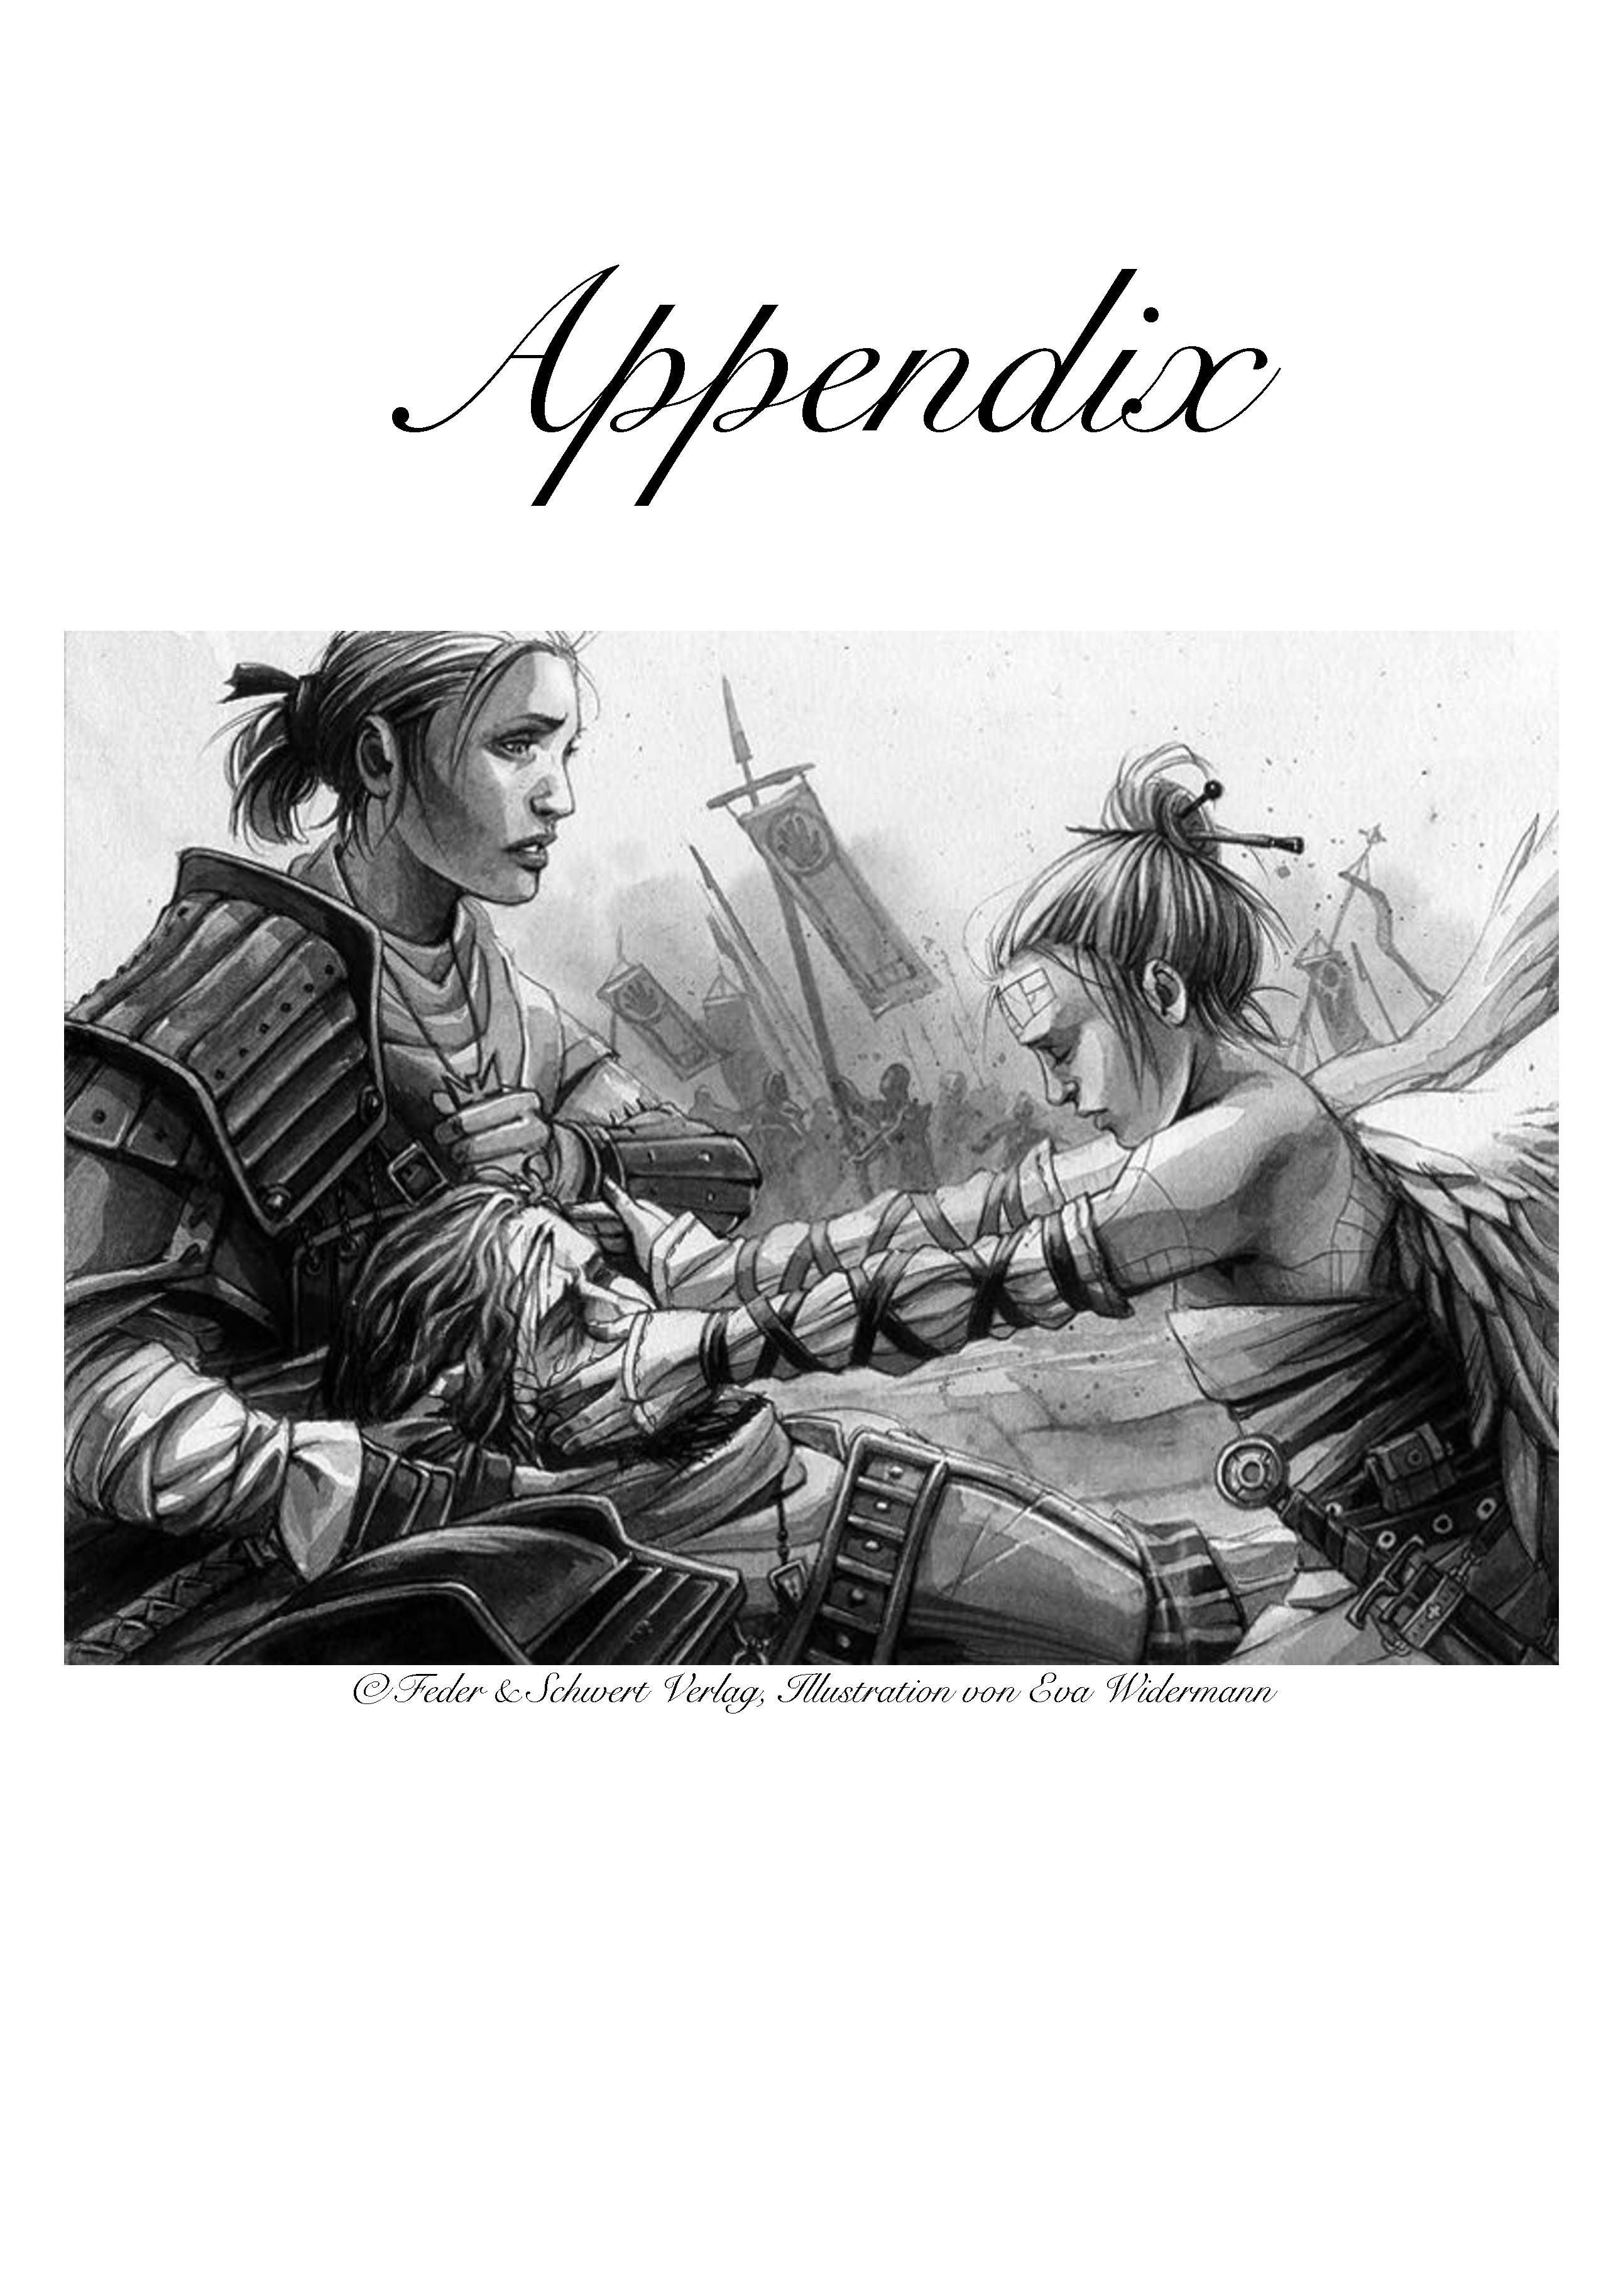
\includepdf{Images/appendixpic.pdf}
\newpage

\chapter{Die 10 Fragen}

Gemäß der gängigen Praxis, sich im Vorfelde Gedanken zu der Herkunft und den Eigenarten seines Charakters zu machen, folgen hier die Antworten auf die zehn Fragen aus dem Grundregelwerk.

\section{Woher kommt Albrecht?}
\enquote{Muss noch ausgespielt werden.}

\section{Wer ist Albrechts Familie?}
%% {Wer ist Albrechts Familie?}

Er wuchs als ältester Sohn zweier Priester auf, welche viele Jahre nach ihm noch ein Mädchen gebaren. Während sein Vater treu der Verena in Ordnungs- und Richtdingen ergeben war, fühlte sich Albrecht schon in jungen Jahren eher seiner Mutter und ihrer Arbeit für den Mórrkult zugehörig.

In seiner Jugend half er ihr immer häufiger, Grab- und Leichenräuber aus den Mórrgärten zu vertreiben und strebte schon seit jungen Jahren eine geistliche Laufbahn im Mórrkult an.

\section{Welcher Gesellschaft gehört er an?}
%% {Welcher Gesellschaft gehört er an?}

Albrecht zählt wegen seiner Tätigkeitezu einer einerseits belächelten und andererseits sehr geschätzten Priestergesellschaft des Shallya Ordens, da umherziehende Wanderpriester für verunglückte Abenteurer manchmal die allerletzte Rettung und damit wahrlich ein Geschenk der Göttin sind.

\section{Was tat Albrecht, ehe er Abenteurer wurde?}
%% {Was tat Albrecht, ehe er Abenteurer wurde?}

Genau genommen sieht er sich überhaupt nicht als Abenteurer. Sein Dienst im Namen Shallyas und die Ordensstrukturen sorgen lediglich dafür, dass er regelmäßig auf Abenteurergruppen trifft und sich ihnen mitunter für längere Jahre anschließt.  
Wichtig ist für ihn nur, so lange Shallyas Lehren zu teilen bis er sich einen Platz in den städtischen Tempeln verdient hat. 


\section{Warum wurde er Abenteurer?}
%% {Warum wurde er Abenteurer?}

Die Wanderpriesterschaft ist eine besondere Eigenart des Shallya Ordens, die verhindern soll, dass die Priesterinnen in den Tempeln ob attraktiver junger Priester gegebenenfalls ihre Aufgaben vernachlässigen könnten.  

Auch wenn diese Restriktion in den Augen vieler Ordensanhänger mittlerweile überholt ist, so hat doch niemand diese Statuen angepasst. Von daher kann Albrecht seiner heilige Pflicht nur auf Wanderschaft nachkommen.  

Dabei sind ihm Abenteuer die liebste Begleitung, weil in sämtlichen Ortschaften die Leiden der Menschen sehr ähnlichsind  und die sechshundertste Kräutermixtur zur Linderung von Verdauungsproblemen langsam ermüdend wird.


\section{Wie religiös ist Albrecht?}
tba

\section{Wer sind seine besten Freunde, wer seine schlimmsten Feinde?}
%% {Wer sind seine besten Freunde, wer seine schlimmsten Feinde?}

Als Wanderpriester halten sich die dauerhaften Kontakte natürlich in Grenzen, weshalb Albrecht keine konkreten Menschen in eine dieser Kategorien stecken kann.

Priestern steht er generell aufgeschlossen und freundlich gegenüber, wohingegen er für Ketzer kaum ein gutes Wort übrig hat.

\section{Welche wertvollen Besitztümer hat Albrecht?}
tba

\section{Wem gegenüber ist er loyal?}
%% {Wem gegenüber ist er loyal?}

Albrechts bedingungslose Loyalität gilt ausschließlich seinem Orden.

Für zweckgebundene Loyalität ist er generell fähig und er wendet sich eigentlich nur von den Gruppen ab, denen er sich anschloss, wenn sie sich über einen \emph{zu} langen Zeitraum \emph{zu} negativ über die Götter geäußert haben.


\section{Wen liebt/hasst Albrecht?}
tba



%% Der Charakterbogen, ohne den doch kein Rollenspiel auskommt
\chapter{Charakterbogen}
Dieser regelmäßig angepasste Charakterbogen dient einerseits dem Spielleiter als Unterstützung und gibt andererseits dem Spieler die Möglichkeit, einen gegebenenfalls vergessenen Charakterbogen lediglich durch Zugriff auf das Internet innerhalb von Minuten zu ersetzen.

Wahnsinn! Wunderwerk der Technik! Schwarze Magie! \emph{Verbrennt ihn!!!}

%% Und nun noch einbinden…
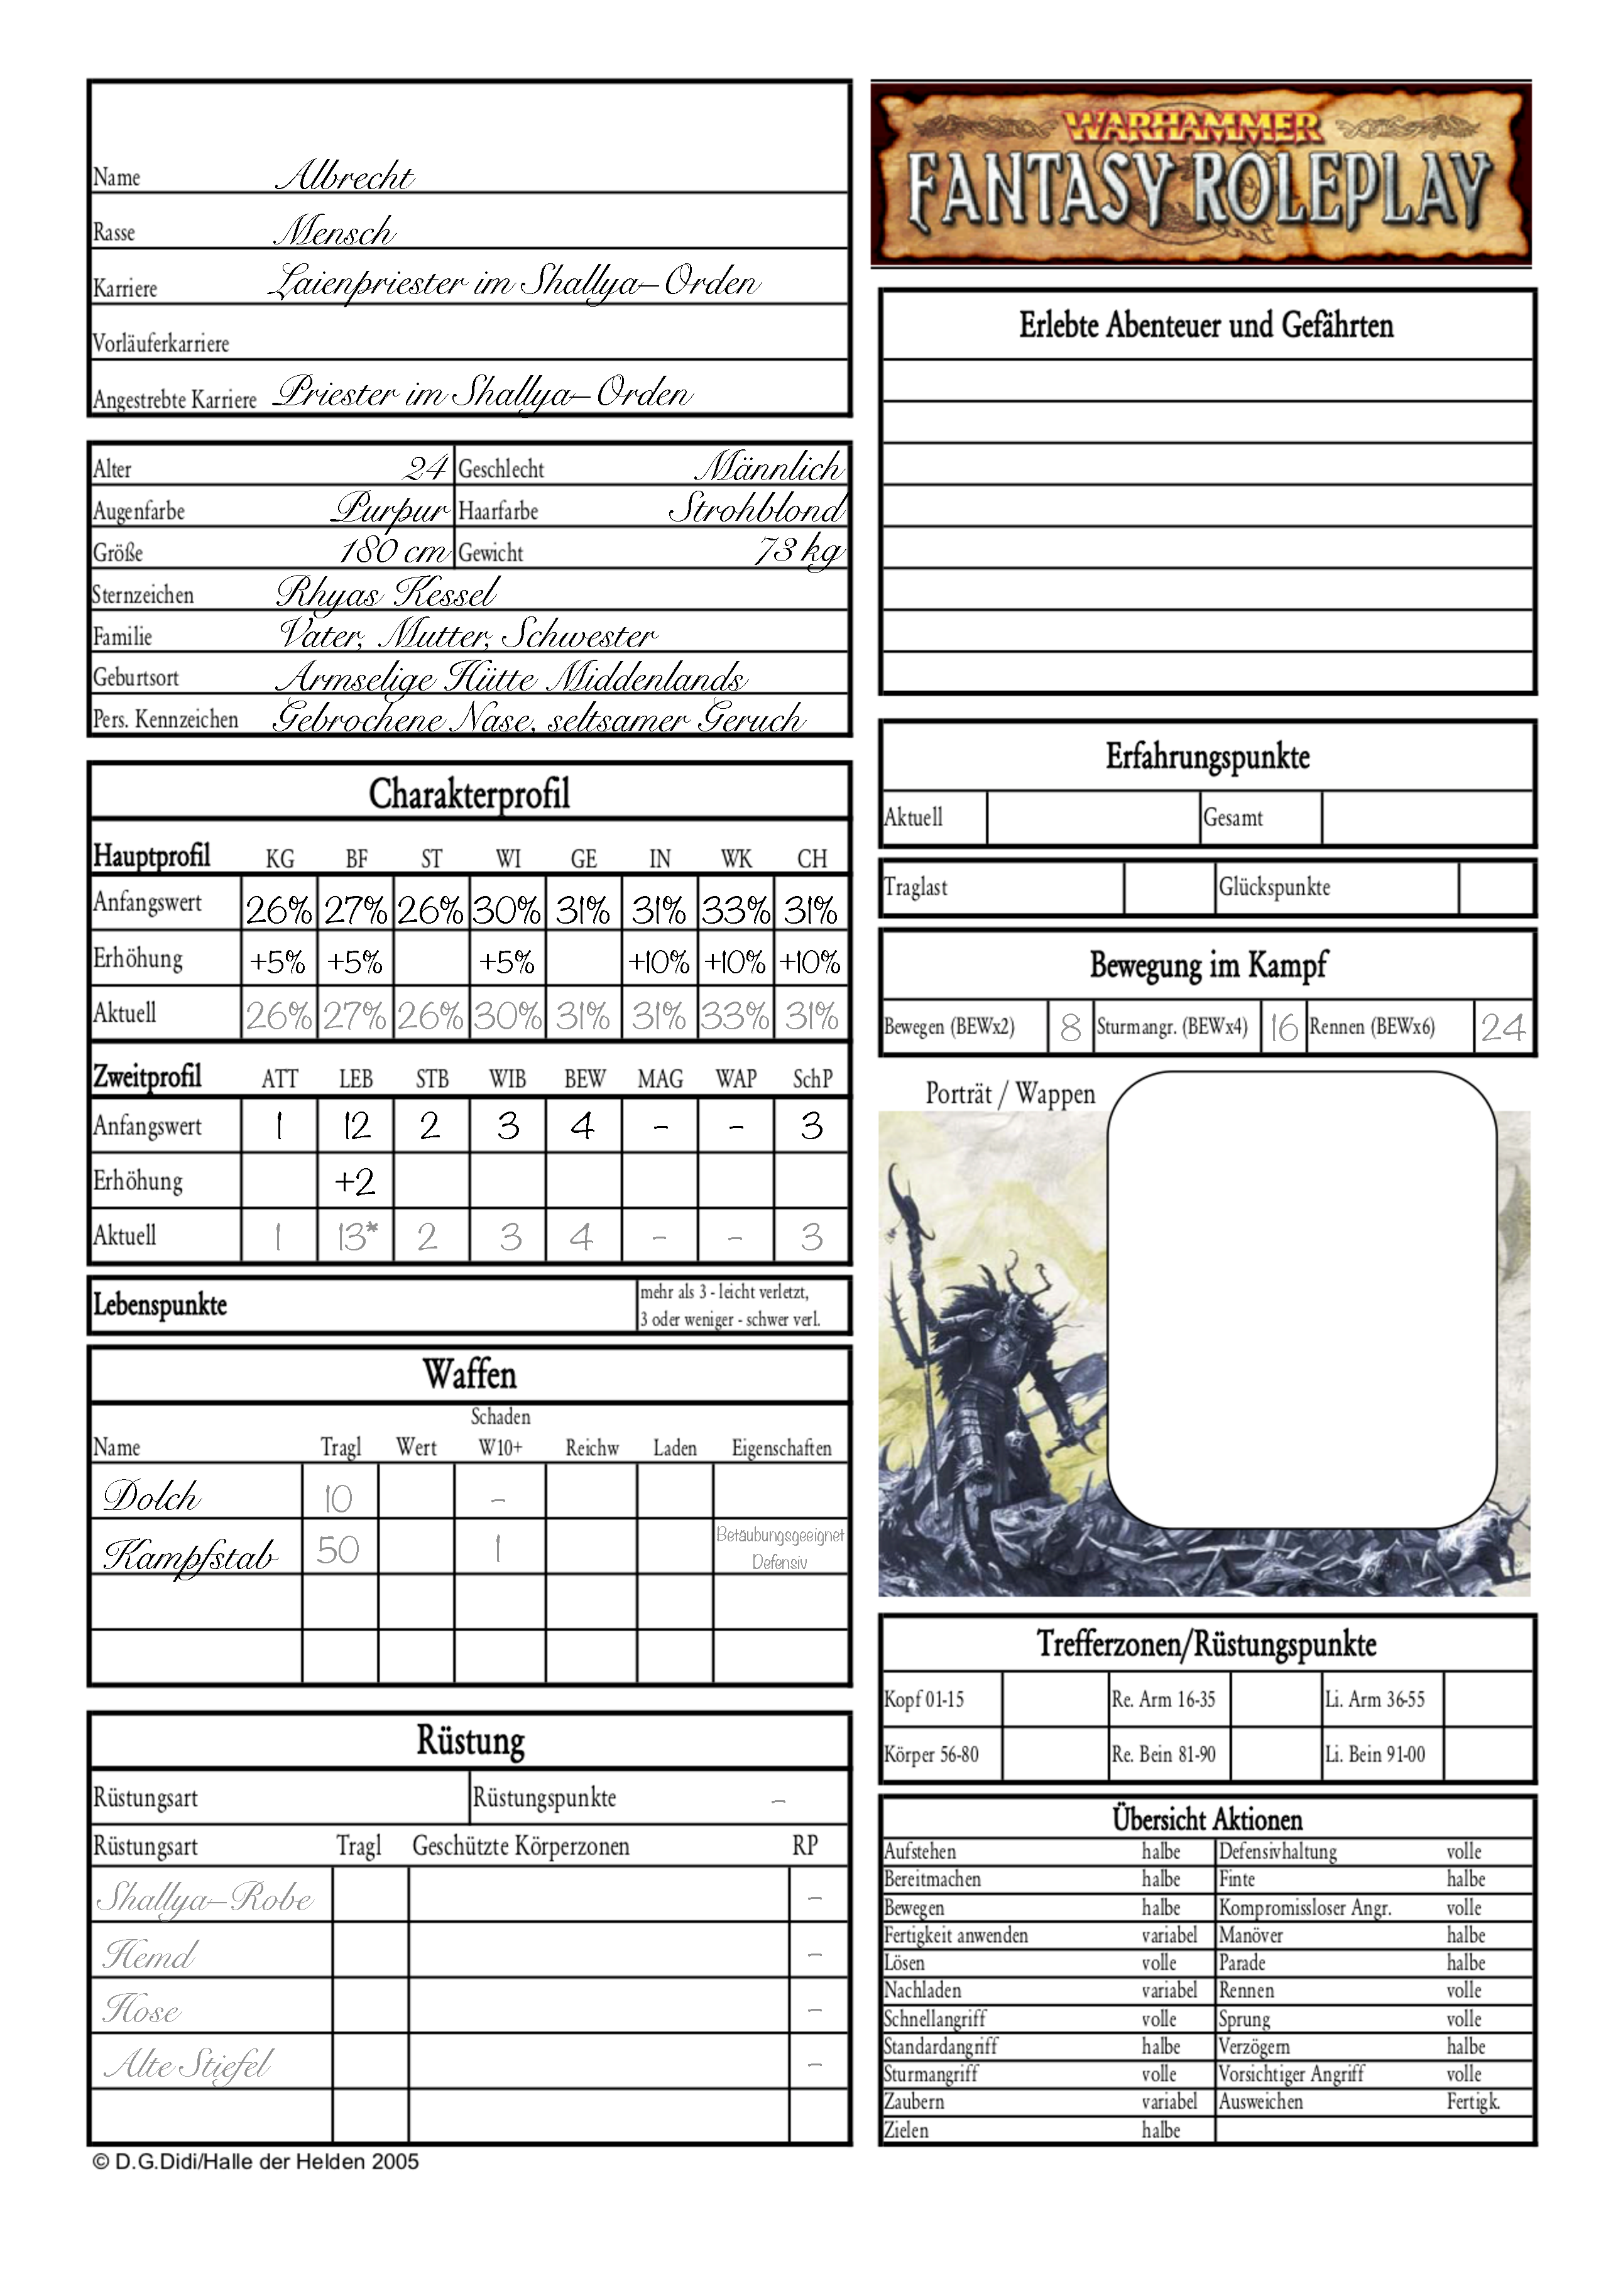
\includepdf[pages=-]{Images/characterbogen_albrecht.pdf}

%% Dokument beenden
\end{document}  